% Created 2016-05-05 四 10:02
\documentclass[xcolor=svgnames,presentation]{beamer}
\usepackage[utf8]{inputenc}
\usepackage[T1]{fontenc}
\usepackage{fixltx2e}
\usepackage{graphicx}
\usepackage{longtable}
\usepackage{float}
\usepackage{wrapfig}
\usepackage{soul}
\usepackage{textcomp}
\usepackage{marvosym}
\usepackage{wasysym}
\usepackage{latexsym}
\usepackage{amssymb}
\usepackage{hyperref}
\tolerance=1000
\usepackage{minted}
\usecolortheme[named=FireBrick]{structure}\setbeamercovered{transparent}\setbeamertemplate{caption}[numbered]\setbeamertemplate{blocks}[rounded][shadow=true] \usetheme{Darmstadt}\date{\today} \usepackage{tikz}\usepackage{xeCJK}\usepackage{amsmath}\setmainfont{Times New Roman}\setCJKmainfont[BoldFont={Adobe Heiti Std},ItalicFont={Adobe Fangsong Std}]{Adobe Heiti Std}\setCJKsansfont{Adobe Heiti Std}\setCJKmonofont{Adobe Fangsong Std}\usepackage{verbatim}\graphicspath{{figures/}} \definecolor{lstbgcolor}{rgb}{0.9,0.9,0.9} \usepackage{listings}\usepackage{minted} \usepackage{fancyvrb}\usepackage{xcolor}\lstset{escapeinside=`',frameround=ftft,language=C,breaklines=true,keywordstyle=\color{blue!70},commentstyle=\color{red!50!green!50!blue!50},frame=shadowbox,backgroundcolor=\color{yellow!20},rulesepcolor=\color{red!20!green!20!blue!20}}
\usemintedstyle{default}
\providecommand{\alert}[1]{\textbf{#1}}

\title{第6讲 Linux磁盘和文件系统管理}
\author{王晓庆}
\date{\today}
\hypersetup{
  pdfkeywords={},
  pdfsubject={},
  pdfcreator={Emacs Org-mode version 7.9.3f}}

\institute{wangxiaoqing@outlook.com}
\begin{document}

\maketitle

\begin{frame}
\frametitle{Outline}
\setcounter{tocdepth}{1}
\tableofcontents
\end{frame}
\section{分区管理}
\label{sec-1}
\begin{frame}
\frametitle{如何使用Linux系统中新添加的磁盘?}
\label{sec-1-1}

\begin{enumerate}
\item 对新磁盘进行分区
\item 在分区上创建文件系统(格式化)
\item 将文件系统挂载到挂载点
\end{enumerate}
\end{frame}
\begin{frame}
\frametitle{创建和管理磁盘分区}
\label{sec-1-2}
\begin{itemize}

\item Linux磁盘设备文件名
\label{sec-1-2-1}%
\begin{itemize}

\item IDE接口设备(由物理连接来区分,一般最多接4个接口)
\label{sec-1-2-1-1}%
\begin{enumerate}
\item /dev/hda \#第1个IDE通道的主设备(master)
\item /dev/hdb \#第1个IDE通道的从设备(slave)
\item /dev/hdc \#第2个IDE通道的主设备(master)
\item /dev/hdd \#第2个IDE通道的从设备(slave)
\end{enumerate}

\item SCSI/SAS/SATA/USB接口设备\\
\label{sec-1-2-1-2}%
IDE磁盘代号只有一个字母,而SCSI磁盘代号可以多达两个字母
\begin{enumerate}
\item /dev/sda   \#第1块SCSI磁盘
\item /dev/sdad  \#第30块SCSI磁盘
\end{enumerate}
\end{itemize} % ends low level
\end{itemize} % ends low level
\end{frame}
\begin{frame}
\frametitle{Linux分区}
\label{sec-1-3}
\begin{itemize}

\item 主引导记录(Master Boot Record, MBR)和分区表\\
\label{sec-1-3-1}%
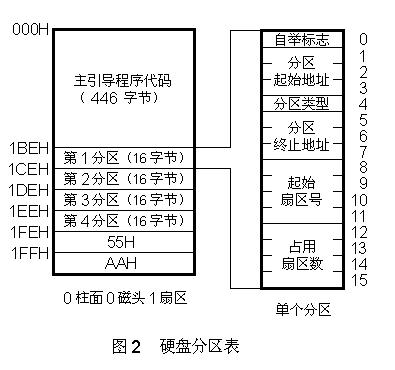
\includegraphics[width=.9\linewidth]{img/mbr.jpg}
\end{itemize} % ends low level
\end{frame}
\begin{frame}[fragile]
\frametitle{Linux分区(2)}
\label{sec-1-4}
\begin{itemize}

\item 查看MBR和分区表\\
\label{sec-1-4-1}%
\begin{minted}[]{bash}
#复制mbr到文件
dd if=/dev/sda of=mbr.dat bs=512 count=1
#查看mbr
hexdump -C mbr.dat
#查看分区表
hexdump -s 446 -n 64 -e \
'1/1 "%02x " 
 3/1 "%02x" 
 1/1 " %02x " 
 3/1 "%02x" " " 
 2/4 "%08x " 
 "\n"' mbr.dat
\end{minted}
\end{itemize} % ends low level
\end{frame}
\begin{frame}
\frametitle{Linux分区(3)}
\label{sec-1-5}
\begin{itemize}

\item 分区表项内容解读\\
\label{sec-1-5-1}%
\begin{center}
\begin{tabular}{rll}
 偏移量  &  长度  &  定义                               \\
\hline
   0x00  &  1B    &  0x00 非活动分区;0x80 活动分区     \\
   0x01  &  1B    &  起始磁头号                         \\
   0x02  &  2B    &  起始扇区号:0x02的低6位            \\
         &        &  起始柱面号:0x02的高2位和0x03字节  \\
   0x04  &  1B    &  文件系统标识:0x83代表Linux分区    \\
   0x05  &  1B    &  结束磁头号                         \\
   0x06  &  2B    &  结束扇区号:0x06的低6位            \\
         &        &  结束柱面号:0x06的高2位和0x07字节  \\
   0x08  &  4B    &  起始逻辑扇区号                     \\
   0x0C  &  4B    &  总扇区数                           \\
\end{tabular}
\end{center}


\end{itemize} % ends low level
\end{frame}
\begin{frame}
\frametitle{Linux分区(4)}
\label{sec-1-6}
\begin{itemize}

\item 分区编号与分区文件名
\label{sec-1-6-1}%
\begin{itemize}

\item IDE磁盘:最多63个分区
\label{sec-1-6-1-1}%

\item SCSI磁盘:最多15个分区
\label{sec-1-6-1-2}%

\item 主分区和扩展分区:1~4
\label{sec-1-6-1-3}%

\item 扩展分区中的逻辑分区:5~15(63)
\label{sec-1-6-1-4}%

\item 例:/dev/sda1, /dev/sdb5
\label{sec-1-6-1-5}%
\end{itemize} % ends low level

\item 分区的文件系统类型
\label{sec-1-6-2}%
\begin{itemize}

\item Linux支持多种文件系统类型
\label{sec-1-6-2-1}%

\item Ext2、Ext3、Ext4、FAT32、FAT16、NTFS、XFS、\ldots{}
\label{sec-1-6-2-2}%

\item swap交换分区
\label{sec-1-6-2-3}%
\end{itemize} % ends low level
\end{itemize} % ends low level
\end{frame}
\begin{frame}[fragile]
\frametitle{利用fdisk进行磁盘分区}
\label{sec-1-7}
\begin{itemize}

\item 查看分区情况\\
\label{sec-1-7-1}%
\begin{minted}[]{bash}
fdisk -l     #按柱面查看分区
fdisk -lu    #按扇区查看分区
\end{minted}

\item 对磁盘进行分区\\
\label{sec-1-7-2}%
\begin{minted}[]{bash}
fdisk /dev/sdb
m  #获取帮助
n  #新增分区
d  #删除分区
p  #打印分区情况
t  #更改分区类型标识
w  #保存退出
q  #不保存退出
partprobe    #不重新启动而让内核重新加载分区表
\end{minted}
\end{itemize} % ends low level
\end{frame}
\section{文件系统管理}
\label{sec-2}
\begin{frame}[fragile]
\frametitle{创建文件系统}
\label{sec-2-1}
\begin{itemize}

\item 使用mkfs创建文件系统\\
\label{sec-2-1-1}%
\begin{minted}[]{bash}
mkfs -t ext3 /dev/sdb1
mkfs.ext3 /dev/sdb1
\end{minted}

\item 使用mke2fs创建文件系统\\
\label{sec-2-1-2}%
\begin{minted}[]{bash}
mke2fs /dev/sdb1
-b  #指定块大小
-j  #创建ext3文件系统
-i  #指定每多少字节分配一个i节点
-N  #直接指定i节点个数
-n  #预览创建结果,并不真正创建
-m  #保留块所占百分比
-L  #指定分区卷标
\end{minted}
\end{itemize} % ends low level
\end{frame}
\begin{frame}[fragile]
\frametitle{管理文件系统}
\label{sec-2-2}
\begin{itemize}

\item 查看文件系统\\
\label{sec-2-2-1}%
\begin{minted}[]{bash}
dumpe2fs /dev/sda1
tune2fs -l /dev/sda1
\end{minted}

\item 调整文件系统\\
\label{sec-2-2-2}%
\begin{minted}[]{bash}
tune2fs -j /dev/sda1        #转换为ext3文件系统
tune2fs -L data /dev/sda1   #设置卷标
blkid /dev/sda1             #查看设备的UUID(128位)
tune2fs -U random /dev/sda1 #设置随机UUID
tune2fs -U clear /dev/sda1  #清除UUID
man tune2fs
\end{minted}

\item 检查/修复文件系统\\
\label{sec-2-2-3}%
\begin{minted}[]{bash}
fsck /dev/sdb1 #fsck应在分区被卸载时运行
\end{minted}
\end{itemize} % ends low level
\end{frame}
\begin{frame}[fragile]
\frametitle{挂载文件系统}
\label{sec-2-3}
\begin{itemize}

\item mount命令\\
\label{sec-2-3-1}%
\begin{minted}[]{bash}
mount [-t type] [-o option] device mountpoint
mount /dev/sda1 /mnt/sda1 #挂载点一般为空目录
mount -a                  #挂载/etc/fstab的文件系统
mount                     #打印文件系统挂载情况
cat /etc/mtab             #同上
mount -t ext2 -o noatime,noexec /dev/sda1 /mnt/sda1
date >/mnt/sda1/date1
mount -o remount,ro /mnt/sda1 #重新挂载已挂载文件系统
date >/mnt/sda1/date2
mount -o remount,rw /mnt/sda1
date >/mnt/sda1/date3
\end{minted}
\end{itemize} % ends low level
\end{frame}
\begin{frame}[fragile]
\frametitle{卸载文件系统}
\label{sec-2-4}
\begin{itemize}

\item umount命令\\
\label{sec-2-4-1}%
卸载文件系统时要确保没有进程在访问该文件系统。

\begin{minted}[]{bash}
fuser /mnt/sda1   #查看正在使用目录的进程
lsof /mnt/sda1    #查看正被进程打开的文件/目录
umount /dev/sda1  #设备名
umount /mnt/sda1  #挂载点
\end{minted}

\item /etc/fstab文件\\
\label{sec-2-4-2}%
\begin{minted}[]{bash}
cat /etc/fstab
man 5 fstab
\end{minted}
\end{itemize} % ends low level
\end{frame}
\begin{frame}[fragile]
\frametitle{访问外部存储设备}
\label{sec-2-5}
\begin{itemize}

\item 挂载/卸载光盘\\
\label{sec-2-5-1}%
\begin{minted}[]{bash}
mkdir /media/cdrom             #创建挂载点
mount /dev/cdrom /media/cdrom  #挂载光盘
umount /dev/cdrom              #卸载光盘
umount /media/cdrom            #同上
eject                          #弹出光驱
eject -t                       #收回光驱
\end{minted}

\item 挂载/卸载USB存储设备\\
\label{sec-2-5-2}%
\begin{minted}[]{bash}
mkdir /media/usb               #创建挂载点
mount -t vfat /dev/sdb1 /media/usb  #挂载
umount /media/usb                   #卸载
\end{minted}
\end{itemize} % ends low level
\end{frame}
\begin{frame}[fragile]
\frametitle{制作和使用光盘镜像文件}
\label{sec-2-6}
\begin{itemize}

\item 从光盘制作镜像文件\\
\label{sec-2-6-1}%
\begin{minted}[]{bash}
cp /dev/cdrom cdrom.iso
\end{minted}

\item 从目录制作镜像文件\\
\label{sec-2-6-2}%
\begin{minted}[]{bash}
mkisofs -r -o mydir.iso mydir
\end{minted}

\item 挂载光盘镜像文件\\
\label{sec-2-6-3}%
\begin{minted}[]{bash}
mkdir /media/iso
mount -o loop cdrom.iso /media/iso
\end{minted}
\end{itemize} % ends low level
\end{frame}
\section{交换空间管理}
\label{sec-3}
\begin{frame}
\frametitle{交换空间}
\label{sec-3-1}
\begin{itemize}

\item 操作系统可在需要时暂时换出部分内存数据至磁盘的交换空间以腾出更多内存空间,或从交换空间将数据换入内存。
\label{sec-3-1-1}%

\item Linux支持两种形式的交换空间
\label{sec-3-1-2}%
\begin{enumerate}
\item 交换分区
\item 交换文件
\end{enumerate}

\item Linux系统最多可以有32个交换空间,386兼容平台上每个交换空间最大不能超过2GB
\label{sec-3-1-3}%

\item 分配交换空间的建议:以4MB或8MB为单位,一般为物理内存1~2倍
\label{sec-3-1-4}%
\end{itemize} % ends low level
\end{frame}
\begin{frame}[fragile]
\frametitle{交换分区}
\label{sec-3-2}


\begin{minted}[]{bash}
#准备:创建分区/dev/sdb1并设置其类型为82(Linux swap)
mkswap /dev/sdb1
free
swapon /dev/sdb1
swapon -s
free
swapoff /dev/sdb1
free
\end{minted}
\end{frame}
\begin{frame}[fragile]
\frametitle{交换文件}
\label{sec-3-3}


\begin{minted}[]{bash}
dd if=/dev/zero of=/tmp/swapfile bs=1M count=200
mkswap /tmp/swapfile
free
swapon /tmp/swapfile
swapon -s
free
swapoff /tmp/swapfile
rm /tmp/swapfile
\end{minted}
\end{frame}
\section{磁盘阵列管理}
\label{sec-4}
\begin{frame}
\frametitle{独立磁盘冗余阵列(Redundant Array of Independent Disks, RAID)}
\label{sec-4-1}

\begin{enumerate}
\item 可以通过并行处理多个独立的I/O请求提高读写性能
\item 可以通过增加冗余信息来提高数据存储的可靠性
\end{enumerate}
\end{frame}
\begin{frame}
\frametitle{RAID 0}
\label{sec-4-2}
\begin{itemize}

\item 非冗余,读写性能好,数据可靠性低于单个磁盘\\
\label{sec-4-2-1}%
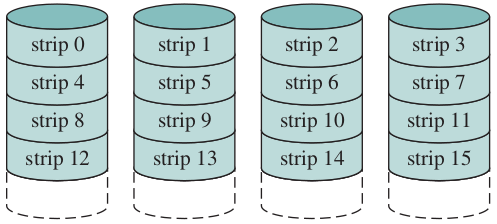
\includegraphics[width=.9\linewidth]{img/raid0.png}
\end{itemize} % ends low level
\end{frame}
\begin{frame}
\frametitle{RAID 1}
\label{sec-4-3}
\begin{itemize}

\item 镜像,读性能好,写性能与单个磁盘相当,数据可靠性高,成本高\\
\label{sec-4-3-1}%
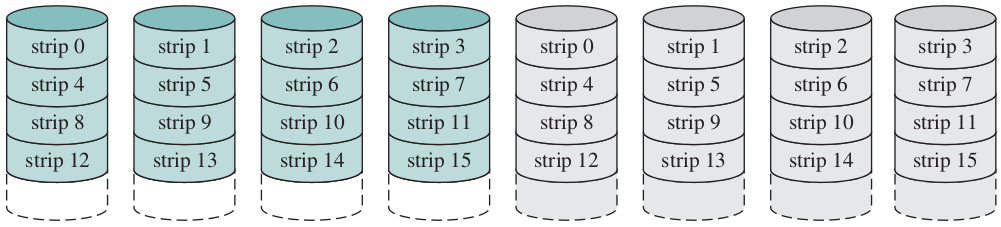
\includegraphics[width=.9\linewidth]{img/raid1.png}
\end{itemize} % ends low level
\end{frame}
\begin{frame}
\frametitle{RAID 2}
\label{sec-4-4}
\begin{itemize}

\item 并行访问,通过海明码实现冗余,读写性能好,磁盘同步旋转,带检错纠错功能,可靠性高,读写性能好,但一次只能执行一个I/O请求\\
\label{sec-4-4-1}%
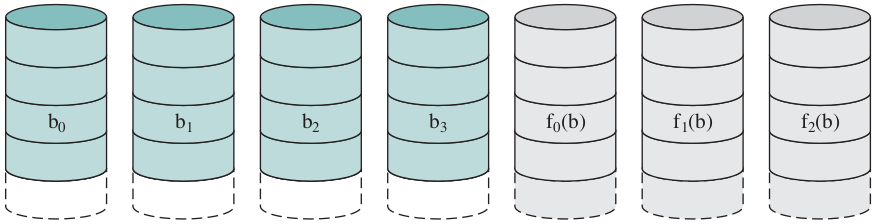
\includegraphics[width=.9\linewidth]{img/raid2.png}
\end{itemize} % ends low level
\end{frame}
\begin{frame}
\frametitle{RAID 3}
\label{sec-4-5}
\begin{itemize}

\item 并性访问,通过奇偶校验实现冗余,读写性能好,磁盘同步旋转,带检错功能,可靠性高,读写性能好,但一次只能执行一个I/O请求\\
\label{sec-4-5-1}%
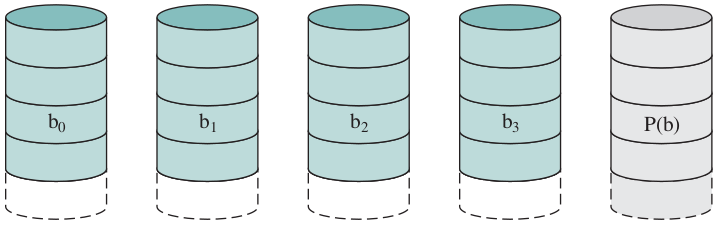
\includegraphics[width=.9\linewidth]{img/raid3.png}
\end{itemize} % ends low level
\end{frame}
\begin{frame}
\frametitle{RAID 4}
\label{sec-4-6}
\begin{itemize}

\item 独立访问,以块为单位计算奇偶校验块并存放与校验盘,数据可靠性高,读性能好,写性能差(因为每次写都要更新校验盘数据),校验盘成为性能瓶颈\\
\label{sec-4-6-1}%
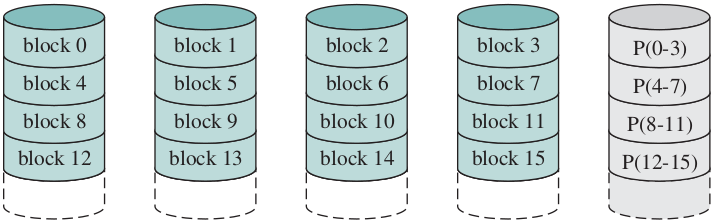
\includegraphics[width=.9\linewidth]{img/raid4.png}
\end{itemize} % ends low level
\end{frame}
\begin{frame}
\frametitle{RAID 5}
\label{sec-4-7}
\begin{itemize}

\item 在RAID 4基础上,把奇偶校验块循环分布在所有磁盘上,从而减轻单个校验盘的性能瓶颈问题,读写性能和可靠性类似于RAID 4\\
\label{sec-4-7-1}%
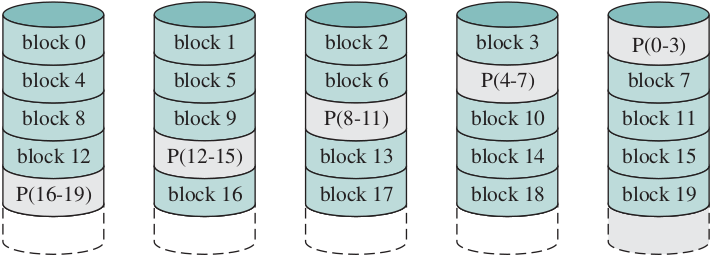
\includegraphics[width=.9\linewidth]{img/raid5.png}
\end{itemize} % ends low level
\end{frame}
\begin{frame}
\frametitle{硬件RAID和软件RAID}
\label{sec-4-8}
\begin{itemize}

\item 硬件RAID
\label{sec-4-8-1}%
\begin{enumerate}
\item 利用硬件RAID控制器来实现,由集成或专用的阵列卡来控制硬盘驱动器
\item 存取性能和数据保护能力高,但成本也高
\item Linux将硬件磁盘阵列看作一块实际的硬盘,其设备名为/dev/sd[a-p]
\end{enumerate}

\item 软件RAID
\label{sec-4-8-2}%
\begin{enumerate}
\item 利用操作系统提供的软件RAID功能来实现
\item 适用于要求不高的场合,成本低
\item Linux将软件磁盘阵列看作多重磁盘设备(MD),其设备名为/dev/md0、/dev/md1等。
\end{enumerate}
\end{itemize} % ends low level
\end{frame}
\begin{frame}[fragile]
\frametitle{利用mdadm管理软件RAID 1阵列(1)}
\label{sec-4-9}
\begin{itemize}

\item 创建RAID 1阵列\\
\label{sec-4-9-1}%
\begin{minted}[]{bash}
#1. 创建两个相同大小的RAID分区,设置分区id为fd
#2. 建立RAID设备
mdadm --create /dev/md0 --level 1 --raid-devices=2 \
/dev/sdb1 /dev/sdc1
#3. 设置mdadm配置文件/etc/mdadm.conf
DEVICE /dev/sdb1 /dev/sdc1
ARRAY /dev/md0 devices=/dev/sdb1,/dev/sdc1
#4. 建立文件系统
mkfs -t ext3 /dev/md0
#5. 挂载RAID 1设备
mkdir /mnt/raid1
mount /dev/md0 /mnt/raid1
\end{minted}
\end{itemize} % ends low level
\end{frame}
\begin{frame}[fragile]
\frametitle{利用mdadm管理软件RAID 1阵列(2)}
\label{sec-4-10}
\begin{itemize}

\item 管理RAID 1阵列\\
\label{sec-4-10-1}%
\begin{minted}[]{bash}
#模拟某成员磁盘发生故障
mdadm /dev/md0 --fail /dev/sdc1
#从RAID 1阵列中移除故障成员
mdadm /dev/md0 --remove /dev/sdc1
#准备一块要替换的磁盘,并将新磁盘加入到阵列中
mdadm /dev/md0 --add /dev/sdd1
#查看阵列实时信息
cat /proc/mdstat
mdadm --detail /dev/md0
\end{minted}
\end{itemize} % ends low level
\end{frame}
\begin{frame}[fragile]
\frametitle{利用mdadm管理软件RAID 5阵列(1)}
\label{sec-4-11}
\begin{itemize}

\item 创建RAID 5阵列\\
\label{sec-4-11-1}%
\begin{minted}[]{bash}
#1. 准备4个阵列成员(创建RAID分区)
#2. 创建RAID设备:系统默认只有md0设备,其他需自行创建
ls –l /dev/md0 #查看md设备的类型和主次设备号
mknod /dev/md1 b 9 1 #创建设备文件
#3. 建立RAID 5设备
mdadm --create /dev/md1 --level=5 \
--raid-devices=3 --spare-devices=1 /dev/sdd[5-8]
mdadm --detail /dev/md1
#4. 设置mdadm配置文件/etc/mdadm.conf
DEVICE /dev/sdd5 /dev/sdd6 /dev/sdd7 /dev/sdd8
ARRAY /dev/md1 devices=/dev/sdd5,/dev/sdd6,/dev/sdd7,/dev/sdd8
mkfs.ext3 /dev/md1 #5. 建立文件系统
mkdir /mnt/raid5
mount /dev/md1 /mnt/raid5 #6. 挂载RAID 5设备
\end{minted}
\end{itemize} % ends low level
\end{frame}
\begin{frame}[fragile]
\frametitle{利用mdadm管理软件RAID 5阵列(2)}
\label{sec-4-12}
\begin{itemize}

\item 管理RAID 5阵列\\
\label{sec-4-12-1}%
\begin{minted}[]{bash}
#利用备用盘重建RAID 5
mdadm /dev/md1 --fail /dev/sdd6
mdadm --detail /dev/md1
#可看到备用盘自动参与重建阵列,而故障盘成为备用磁盘,而且表示出故障状态
#注意:要等待RAID重建完毕,再替换故障磁盘
#将故障磁盘移除并加入新磁
mdadm /dev/md1 --remove /dev/sdd6
mdadm /dev/md1 --add /dev/sde1
mdadm --detail /dev/md1
\end{minted}
\end{itemize} % ends low level
\end{frame}
\begin{frame}[fragile]
\frametitle{利用mdadm管理软件RAID}
\label{sec-4-13}
\begin{itemize}

\item 启用/停用/监控RAID设备\\
\label{sec-4-13-1}%
\begin{minted}[]{bash}
#停止RAID设备(停止前要先卸载)
mdadm --stop /dev/md0
#启动RAID设备
mdadm --assemble --scan /dev/md0
#监控RAID设备
mdadm --monitor --mail=admin@abc.com \
--delay=180 /dev/md0
#将监控任务转入后台执行
nohup mdadm --monitor --mail=admin@abc.com \
--delay=180 /dev/md0
\end{minted}
\end{itemize} % ends low level
\end{frame}
\begin{frame}[fragile]
\frametitle{利用mdadm管理软件RAID}
\label{sec-4-14}
\begin{itemize}

\item 删除RAID多重磁盘设备\\
\label{sec-4-14-1}%
每个md设备只能被建立一次,如果创建命令(mdadm --create)出错,将造成该md设备无法使用,这时需要按以下步骤先删除该错误的md设备,然后才能重新创建它。

\begin{minted}[]{bash}
#1. 停用RAID设备
mdadm --stop /dev/md0
#2. 清空每个组成分区的超级块
mdadm --zero-superblock /dev/sdb1
mdadm --zero-superblock /dev/sdc1
\end{minted}
\end{itemize} % ends low level
\end{frame}
\section{逻辑卷管理}
\label{sec-5}
\begin{frame}
\frametitle{简介}
\label{sec-5-1}
\begin{itemize}

\item 服务器大多处于要求具备高可用性的运行环境,调整磁盘存储空间有时不允许重新引导系统,逻辑卷可以在系统处于运行状态时扩充和缩减,可为管理员提供磁盘存储管理的灵活性。
\label{sec-5-1-1}%
\end{itemize} % ends low level
\end{frame}
\begin{frame}
\frametitle{逻辑卷体系结构}
\label{sec-5-2}

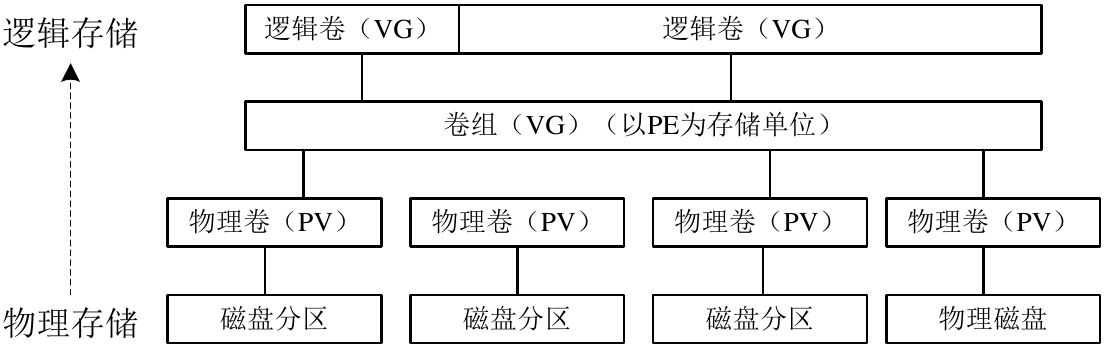
\includegraphics[width=.9\linewidth]{img/lvm.png}
\end{frame}
\begin{frame}
\frametitle{逻辑卷管理工具}
\label{sec-5-3}
\begin{itemize}

\item 创建逻辑卷步骤
\label{sec-5-3-1}%
\begin{enumerate}
\item 创建物理卷(PV)
\item 创建卷组(VG):卷组以大小相等的区域(PE)为单位分配存储容量
\item 创建逻辑卷(LV)
\end{enumerate}

\item lvm2:提供了一组工具用于管理逻辑卷\\
\label{sec-5-3-2}%
\begin{center}
\begin{tabular}{llll}
 功能          &  物理卷     &  卷组       &  逻辑卷              \\
\hline
 扫描检测      &  pvscan     &  vgscan     &  lvscan              \\
 显示详细信息  &  pvdisplay  &  vgdisplay  &  lvdisplay           \\
 创建          &  pvcreate   &  vgcreate   &  lvcreate            \\
 删除          &  pvremove   &  vgremove   &  lvremove            \\
 扩充          &             &  vgextend   &  lvextend(lvresize)  \\
 缩减          &             &  vgreduce   &  lvreduce(lvresize)  \\
 改变属性      &  pvchange   &  vgchange   &  lvchange            \\
\end{tabular}
\end{center}


\end{itemize} % ends low level
\end{frame}
\begin{frame}[fragile]
\frametitle{建立逻辑卷(1)}
\label{sec-5-4}
\begin{itemize}

\item 1. 建立物理卷\\
\label{sec-5-4-1}%
\begin{minted}[]{bash}
#创建磁盘分区(100柱面大小),并将分区的ID设为8e
pvcreate /dev/sdb2 /dev/sdb3     #建立物理卷
pvscan                           #扫描物理卷信息
pvs                              #查看物理卷简要信息
pvdisplay                        #查看物理卷详细信息
\end{minted}

\item 2. 建立卷组\\
\label{sec-5-4-2}%
\begin{minted}[]{bash}
vgcreate -s 16M vg1 /dev/sdb[23] #创建卷组
#-s指定PE大小,默认为4M,最小为1K,且必须为2的次幂
vgs                              #显示卷组简要信息
vgdisplay                        #显示卷组详细信息
\end{minted}
\end{itemize} % ends low level
\end{frame}
\begin{frame}[fragile]
\frametitle{建立逻辑卷(2)}
\label{sec-5-5}
\begin{itemize}

\item 3. 建立逻辑卷\\
\label{sec-5-5-1}%
\begin{minted}[]{bash}
lvcreate -l 7500 -n lv1 vg1      #创建逻辑卷
lvcreate -L 1200M -n lv1 vg1    #同上
#-l指定PE数量,-L指定容量(k,m,g,t,不区分大小写)
lvs                             #显示逻辑卷简要信息
lvdisplay                       #显示逻辑卷详细信息
\end{minted}

\item 4. 使用逻辑卷\\
\label{sec-5-5-2}%
\begin{minted}[]{bash}
mkfs -t ext3 /dev/vg1/lv1       #建立文件系统
mkdir /mnt/lvm1
mount /dev/vg1/lv1 /mnt/lv1     #挂载逻辑卷
mount /dev/mapper/vg1-lv1 /mnt/lv1   #同上
#创建文件测试
dd if=/dev/zero of=/mnt/lv1/bigfile bs=1M count=800
ls /mnt/lv1
df -h /mnt/lv1
\end{minted}
\end{itemize} % ends low level
\end{frame}
\begin{frame}[fragile]
\frametitle{动态调整逻辑卷容量(1)}
\label{sec-5-6}
\begin{itemize}

\item 放大:先放大逻辑卷,再放大文件系统\\
\label{sec-5-6-1}%
\begin{minted}[]{bash}
pvcreate /dev/sdb5             #新建物理卷
vgextend vg1 /dev/sdb5         #扩充卷组
vgdisplay vg1                  #显示卷组信息
lvdisplay /dev/vg1/lv1         #显示逻辑卷信息
lvresize -l +50  /dev/vg1/lv1  #扩充逻辑卷
lvresize -L +800M /dev/vg1/lv1 #扩充逻辑卷
lvdisplay /dev/vg1/lv1         #显示卷组信息
df -h /mnt/lv1                 #查看逻辑卷空间情况
resize2fs /dev/vg1/lv1         #扩充文件系统
df -h /mnt/lv1                 #查看逻辑卷空间情况
\end{minted}
\end{itemize} % ends low level
\end{frame}
\begin{frame}[fragile]
\frametitle{动态调整逻辑卷容量(2)}
\label{sec-5-7}
\begin{itemize}

\item 缩小:先缩小文件系统,再缩小逻辑卷(操作需谨慎,注意事先备份数据)\\
\label{sec-5-7-1}%
\begin{minted}[]{bash}
dh -h /mnt/lv1              #查看逻辑卷空间情况
umount /mnt/lv1             #卸载逻辑卷
e2fsck -f /dev/vg1/lv1      #检查逻辑卷
resize2fs /dev/vg1/lv1 1G   #缩小文件系统
lvreduce -L 1G /dev/vg1/lv1 #缩小逻辑卷
lvs                         #查看逻辑卷简要信息
mount /dev/vg1/lv1 /mnt/lv1 #重新挂载逻辑卷
dh -h /mnt/lv1              #查看逻辑卷空间情况
\end{minted}
\end{itemize} % ends low level
\end{frame}
\begin{frame}[fragile]
\frametitle{动态调整卷组}
\label{sec-5-8}
\begin{itemize}

\item 动态替换物理卷\\
\label{sec-5-8-1}%
\begin{minted}[]{bash}
#替换
pvcreate /dev/sdb6         #创建新物理卷
vgextend vg1 /dev/sdb6     #向卷组添加物理卷
vgs -o+pv_used             #查看物理卷信息
pvmove /dev/sdb2 /dev/sdb6 #转移物理卷数据
vgreduce vg1 /dev/sdb2     #从卷组中删除物理卷
vgs -o+pv_used
ls /mnt/lv1
#恢复
pvextend vg1 /dev/sdb2
pvmove /dev/sdb6 /dev/sdb2
vgreduce vg1 /dev/sdb6
vgs -o+pv_used
ls /mnt/lv1
\end{minted}
\end{itemize} % ends low level
\end{frame}
\begin{frame}[fragile]
\frametitle{删除lvm}
\label{sec-5-9}
\begin{itemize}

\item 要删除逻辑卷并恢复磁盘分区,可执行建立逻辑卷的逆过程:\\
\label{sec-5-9-1}%
\begin{minted}[]{bash}
#1. 卸载逻辑卷
umount /mnt/lv1
#2. 删除逻辑卷
lvremove /dev/vg1/lv1
#3. 停用卷组
vgchange -a n vg1
#4. 删除卷组
vgremove vg1
#5. 删除物理卷
pvremove /dev/sde[23]
#6. 使用fdisk将分区ID改回83
\end{minted}
\end{itemize} % ends low level
\end{frame}
\section{磁盘配额管理}
\label{sec-6}
\begin{frame}
\frametitle{磁盘配额}
\label{sec-6-1}
\begin{itemize}

\item 多个用户共享同一磁盘空间时,为防止某用户(组)占用过多磁盘空间,可通过设置磁盘配额(Disk Quota)对其可用存储空间进行限制。
\label{sec-6-1-1}%

\item Linux磁盘配额软件(quota)的特点
\label{sec-6-1-2}%
\begin{enumerate}
\item 只能对分区进行设置,不能对目录进行设置
\item 可以针对用户设置,也可针对组设置
\item 磁盘配额只适用于普通用户或组,root用户不受其限制
\end{enumerate}

\item 在Linux系统中磁盘配额的限制项目有两种类型
\label{sec-6-1-3}%
\begin{enumerate}
\item 磁盘容量限制:限制用户能够使用的磁盘块数(block),实际应用中多使用此类型
\item 文件数量限制:限制用户能够使用的索引节点数(inode),即文件数
\end{enumerate}
\end{itemize} % ends low level
\end{frame}
\begin{frame}[fragile]
\frametitle{启用和管理磁盘配额}
\label{sec-6-2}


\begin{minted}[]{bash}
#1. 修改/etc/fstab配置文件
/dev/sdb1 /mnt/sdb1 ext3 defaults,usrquota,grpquota 0 0
#2. 重新挂载分区
mount -o remount /mnt/sdb1
mount
#3. 扫描分区并生成磁盘配额信息文件
quotacheck -cvuga   #/etc/fstab中设定了配额选项的分区
quotacheck -cvug /mnt/sdb1 #指定分区
ls /mnt/sdb1
#4. 启用磁盘配额
quotaon -a
quotaon /mnt/sdb1
#5. 编辑用户/组配额
edquota mike
edquota -g stu
\end{minted}
\note{说明

\begin{enumerate}
\item edquota中只有软限制和硬限制可以修改,当前的使用量不能修改
\item 指定用户必须在指定分区内有写权限
\item 只有指定用户在磁盘上拥有文件/目录后,quota命令才会显示该用户的磁盘配额情况
\item block是以KB为单位进行分配的
\end{enumerate}
}
\end{frame}
\begin{frame}[fragile]
\frametitle{设置磁盘配额}
\label{sec-6-3}
\begin{columns}
\begin{column}{0.5\textwidth}
%% 左
\label{sec-6-3-1}
\begin{itemize}

\item 配置磁盘配额限制值
\label{sec-6-3-2}%
\begin{itemize}

\item 硬限制(hard)
\label{sec-6-3-2-1}%

\item 软限制(soft)
\label{sec-6-3-2-2}%

\item 软限制宽限期\\
\label{sec-6-3-2-3}%
\begin{minted}[]{bash}
edquota -t
\end{minted}
\end{itemize} % ends low level

\item 复制配额设置\\
\label{sec-6-3-3}%
\begin{minted}[]{bash}
#复制mike的配额设置
edquota -p mike mary bob
\end{minted}
\end{itemize} % ends low level
\end{column}
\begin{column}{0.5\textwidth}
%% 右
\label{sec-6-3-4}

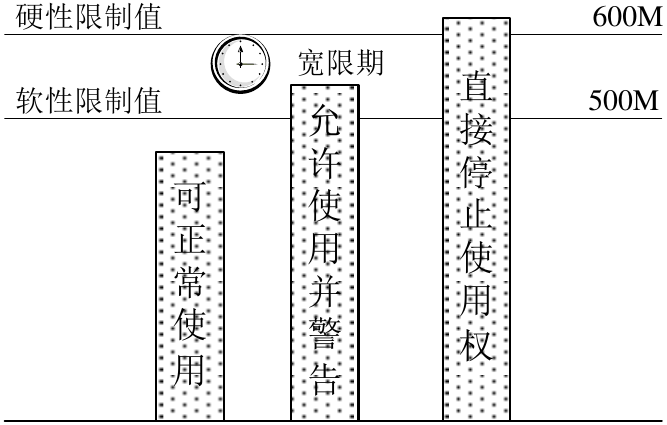
\includegraphics[width=.9\linewidth]{img/quota.png}
\end{column}
\end{columns}
\end{frame}
\section{备份管理}
\label{sec-7}
\begin{frame}
\frametitle{备份内容}
\label{sec-7-1}
\begin{itemize}

\item 系统数据备份\\
\label{sec-7-1-1}%
备份操作系统和应用程序,以便在系统崩溃后能恢复系统运行。

\item 用户数据备份\\
\label{sec-7-1-2}%
备份用户的数据文件,以便用户恢复自己丢失或损坏的数据。

\item 用户的数据变动相对频繁,因此,用户备份应该比系统备份更加频繁。可采用自动定期运行某个程序的方法来备份数据。
\label{sec-7-1-3}%
\end{itemize} % ends low level
\end{frame}
\begin{frame}
\frametitle{备份原理}
\label{sec-7-2}
\begin{itemize}

\item 备份标识
\label{sec-7-2-1}%
\begin{itemize}

\item 当一个文件被备份后,该文件会获得一个“已备份”属性,而当文件属性和内容发生变化时,文件的“已备份”属性将被清除。当备份时,就是依据文件的“已备份”属性来确定要备份哪些文件的。
\label{sec-7-2-1-1}%
\end{itemize} % ends low level
\end{itemize} % ends low level
\end{frame}
\begin{frame}
\frametitle{备份方式}
\label{sec-7-3}
\begin{itemize}

\item 完全备份(Full Backup)
\label{sec-7-3-1}%
\begin{itemize}

\item 对系统进行一次全面的备份,并将所有文件标识为“已备份”
\label{sec-7-3-1-1}%

\item 所需时间最长,但恢复时间最短,操作最方便
\label{sec-7-3-1-2}%
\end{itemize} % ends low level

\item 增量备份(Incremental Backup)
\label{sec-7-3-2}%
\begin{itemize}

\item 只对上一次备份后增加的和修改过的数据进行备份,并添加“已备份”标识
\label{sec-7-3-2-1}%

\item 可快速完成备份,但可靠性较差,恢复较麻烦
\label{sec-7-3-2-2}%
\end{itemize} % ends low level

\item 差异备份(Differential Backup)
\label{sec-7-3-3}%
\begin{itemize}

\item 只对上一次完全备份后增加和修改或的数据进行备份,但不添加“已备份”标识
\label{sec-7-3-3-1}%

\item 所需时间较短,且恢复较为方便,适合各种场合
\label{sec-7-3-3-2}%
\end{itemize} % ends low level
\end{itemize} % ends low level
\end{frame}
\begin{frame}
\frametitle{备份规划}
\label{sec-7-4}
\begin{itemize}

\item 单纯的完全备份
\label{sec-7-4-1}%
\begin{itemize}

\item 适合数据量不大或者数据变动频率很高的情况
\label{sec-7-4-1-1}%
\end{itemize} % ends low level

\item 完全备份结合增量备份
\label{sec-7-4-2}%
\begin{itemize}

\item 以较长周期进行完全备份,其间则进行较短周期增量备份
\label{sec-7-4-2-1}%

\item 如每周一次完全备份结合每日一次增量备份
\label{sec-7-4-2-2}%
\end{itemize} % ends low level

\item 完全备份结合差异备份
\label{sec-7-4-3}%
\begin{itemize}

\item 以较长周期进行完全备份,其间则进行较短周期差异备份
\label{sec-7-4-3-1}%

\item 如每周一次完全备份结合每日一次差异备份\\
\label{sec-7-4-3-2}%
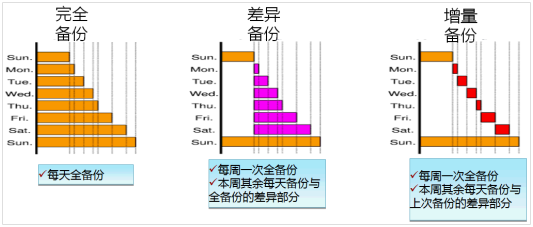
\includegraphics[width=.9\linewidth]{img/backup2.jpg}
\end{itemize} % ends low level
\end{itemize} % ends low level
\end{frame}
\begin{frame}
\frametitle{数据备份操作}
\label{sec-7-5}
\begin{itemize}

\item tar备份
\label{sec-7-5-1}%

\item dump和restore工具
\label{sec-7-5-2}%

\item 光盘备份
\label{sec-7-5-3}%
\end{itemize} % ends low level
\end{frame}
\begin{frame}
\frametitle{dump和restore工具(1)}
\label{sec-7-6}
\begin{itemize}

\item 使用dump和restore实现备份和恢复
\label{sec-7-6-1}%
\begin{itemize}

\item dump能备份任何类型的文件甚至设备,支持完全、增量和差异备份\\
\label{sec-7-6-1-1}%
注意:dump只能对分区进行增量备份和差异备份,对目录只能进行完全备份

\item dump需要指定一个备份级别,它是0-9之间的一个整数
\label{sec-7-6-1-2}%

\item 级别0代表完全备份
\label{sec-7-6-1-3}%

\item 级别n(n>0)代表基于最近一次低于级别n的备份进行差异备份
\label{sec-7-6-1-4}%
\end{itemize} % ends low level
\end{itemize} % ends low level
\end{frame}
\begin{frame}[fragile]
\frametitle{dump和restore工具(2)}
\label{sec-7-7}
\begin{itemize}

\item 使用dump实现完全备份\\
\label{sec-7-7-1}%
\begin{minted}[]{bash}
dump -0S /dev/sda1  #计算完全备份/dev/sda1所需空间
#完全备份/boot分区
dump -0u -f /tmp/boot.dump /boot
dump -0uj -f /tmp/boot.dump.bz2 /boot
#-u 表示更新数据库文件/etc/dumpdates
#   (记录文件日期、存储级别、文件系统等信息)
#-f 指定备份文件
#-j 用bzip2进行压缩
dump -W  #查看分区备份情况
\end{minted}
\end{itemize} % ends low level
\end{frame}
\begin{frame}[fragile]
\frametitle{dump和restore工具(3)}
\label{sec-7-8}
\begin{itemize}

\item 使用dump实现完全备份和增量备份\\
\label{sec-7-8-1}%
\begin{minted}[]{bash}
dump -0u -f /tmp/boot0.dump /boot
dump -1u -f /tmp/boot1.dump /boot
dump -2u -f /tmp/boot2.dump /boot
dump -3u -f /tmp/boot3.dump /boot
\end{minted}

\item 使用dump实现完全备份和差异备份\\
\label{sec-7-8-2}%
\begin{minted}[]{bash}
dump -0u -f /tmp/boot0.dump /boot
dump -1u -f /tmp/boot1.dump /boot
dump -1u -f /tmp/boot2.dump /boot
dump -1u -f /tmp/boot3.dump /boot
\end{minted}
\end{itemize} % ends low level
\end{frame}
\begin{frame}[fragile]
\frametitle{dump和restore工具(4)}
\label{sec-7-9}
\begin{itemize}

\item 使用restore恢复备份\\
\label{sec-7-9-1}%
\begin{minted}[]{bash}
#比较备份文件与文件系统之间的差异
restore –C f /tmp/boot.dump
#恢复之前,浏览备份文件的数据
restore -tf /tmp/boot.dump
#恢复备份(restore不支持覆盖式还原,应还原至其他位置)
mkdir bootbak
cd bootbak
restore -rf /tmp/boot.dump
#-r 表示重建
#进入交互式恢复模式
restore -if /tmp/boot.dump
\end{minted}
\end{itemize} % ends low level
\end{frame}
\begin{frame}[fragile]
\frametitle{光盘备份}
\label{sec-7-10}
\begin{itemize}

\item 建立光盘映像文件\\
\label{sec-7-10-1}%
\begin{minted}[]{bash}
mkisofs -r -o /tmp/boot.iso /boot
#-r 支持长文件名,-o 指定输出文件
dd if=/dev/sda1 of=/tmp/boot.iso
\end{minted}

\item 刻录光盘\\
\label{sec-7-10-2}%
\begin{minted}[]{bash}
cdrecord -scanbus dev=ATA #获取刻录机设备识别号
cdrecord -v dev=ATA:0,1,0 boot.iso  #刻录
cdrecord -v -eject speed=8 dev=ATA:0,1,0 boot.iso #刻录
#-v 输出尽可能多的校验信息
#-eject 刻录完毕后弹出光盘
#speed=8 指定刻录机的速度
\end{minted}

\end{itemize} % ends low level
\end{frame}

\end{document}
